\section{Simulation Results}
\label{sec:simulation}

Fig.~\ref{fig:pn} shows the conceptual phase noise profiles at key nodes.
The \SI{35}{\giga\hertz} input trace follows a combined flicker-plus-white
noise model. The ideal doubled output sits \SI{6}{\decibel} above the input
in accordance with \eqref{eq:6dB}. The free-running \SI{70}{\giga\hertz}
doubler exhibits a noisier profile with a \SI{50}{\mega\hertz} noise corner;
injection locking pulls it to the ideal $+6\,\mathrm{dB}$ bound within the
locking bandwidth $f_L$, beyond which it tracks its free-running noise floor.

\begin{figure*}[t]
\centering
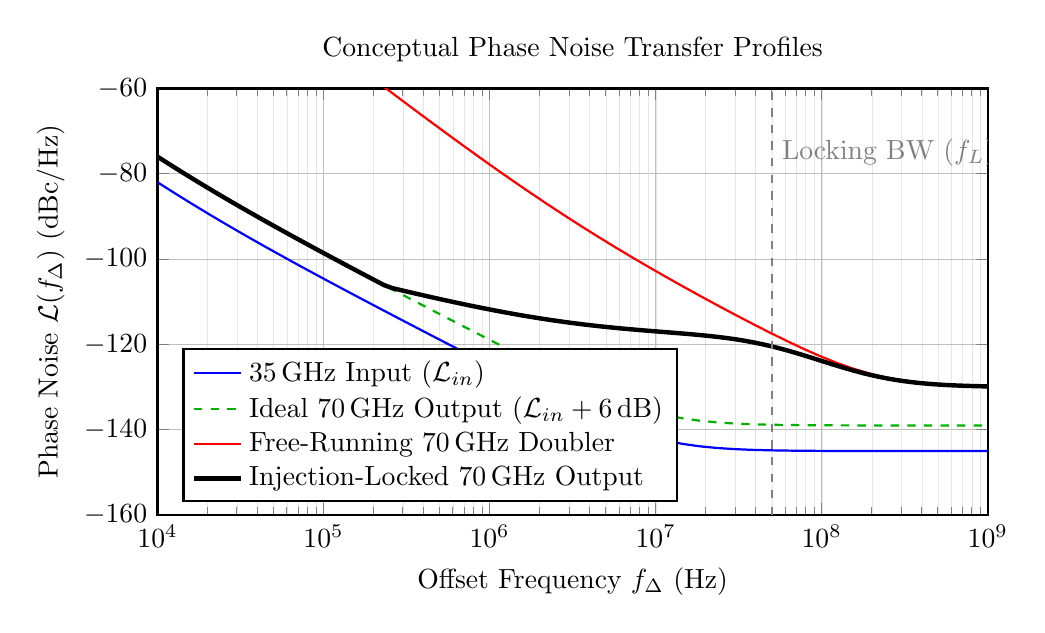
\begin{tikzpicture}
\begin{axis}[
    width=\linewidth,
    height=7cm,
    xmode=log,
    xmin=1e4, xmax=1e9,
    ymin=-160, ymax=-60,
    grid=both,
    grid style={line width=.1pt, draw=gray!20},
    major grid style={line width=.2pt, draw=gray!50},
    xlabel={Offset Frequency $f_\Delta$ (Hz)},
    ylabel={Phase Noise $\mathcal{L}(f_\Delta)$ (dBc/Hz)},
    title={Conceptual Phase Noise Transfer Profiles},
    legend pos=south west,
    legend cell align={left},
    thick
]
    \addplot[blue, domain=1e4:1e9, samples=50]
        {-145 + 10*log10(1 + (1e6/x)^3 + (1e7/x)^2)};
    \addlegendentry{35\,GHz Input ($\mathcal{L}_{in}$)}

    \addplot[green!70!black, dashed, domain=1e4:1e9, samples=50]
        {-139 + 10*log10(1 + (1e6/x)^3 + (1e7/x)^2)};
    \addlegendentry{Ideal 70\,GHz Output ($\mathcal{L}_{in}+6\,\mathrm{dB}$)}

    \addplot[red, domain=1e4:1e9, samples=50]
        {-130 + 10*log10(1 + (5e7/x)^3 + (2e8/x)^2)};
    \addlegendentry{Free-Running 70\,GHz Doubler}

    \addplot[black, ultra thick, domain=1e4:1e9, samples=100]
        {max(
            -139 + 10*log10(1 + (1e6/x)^3 + (1e7/x)^2),
            -130 + 10*log10(1 + (5e7/x)^3 + (2e8/x)^2)
                  - 10*log10(1 + (5e7/x)^2)
        )};
    \addlegendentry{Injection-Locked 70\,GHz Output}

    \draw[dashed, thick, gray]
        (axis cs:5e7,-160) -- (axis cs:5e7,-60)
        node[pos=0.85, right] {Locking BW ($f_L$)};
\end{axis}
\end{tikzpicture}
\caption{Conceptual phase noise at the \SI{35}{\giga\hertz} input,
         the ideal doubled output ($+6\,\mathrm{dB}$), the free-running
         doubler, and the injection-locked output. Within the locking
         bandwidth $f_L \approx \SI{50}{\mega\hertz}$ the output tracks the
         ideal curve; beyond $f_L$ it reverts to the free-running profile.}
\label{fig:pn}
\end{figure*}

% TODO: post-layout simulation results (INL/DNL, phase step uniformity)
